\section{\MBSim - Program Overview}
From the software development point of view, \cite{Sch97} proposed a standard structure for multibody simulation frameworks distinguishing between bodies and interactions. The programs described in \cite{Aca07} and \cite{Ber07} follow also this approach. It is approved and also used in \emph{MBSim} using the object-oriented C++ programming style. The interface of all classes is documented in the source code using Doxygen. This documentation has been extracted for convenient study together with a class overview during installation with the command \texttt{make doc}. Just change to \texttt{\$HOME/MBSim/*/doc/html} and open \texttt{index.html} with an appropriate browser. With this class documentation and the use of self-explaining names in the user interface it is goal of this section to give an overview about the main features of \MBSim{}.\par

Figure~\ref{fig:departure:mbsim:embedding} shows the embedding of \emph{MBSim} in the global simulation and analysing process. 
\begin{figure}[hbt]%
	\centering
    \footnotesize
    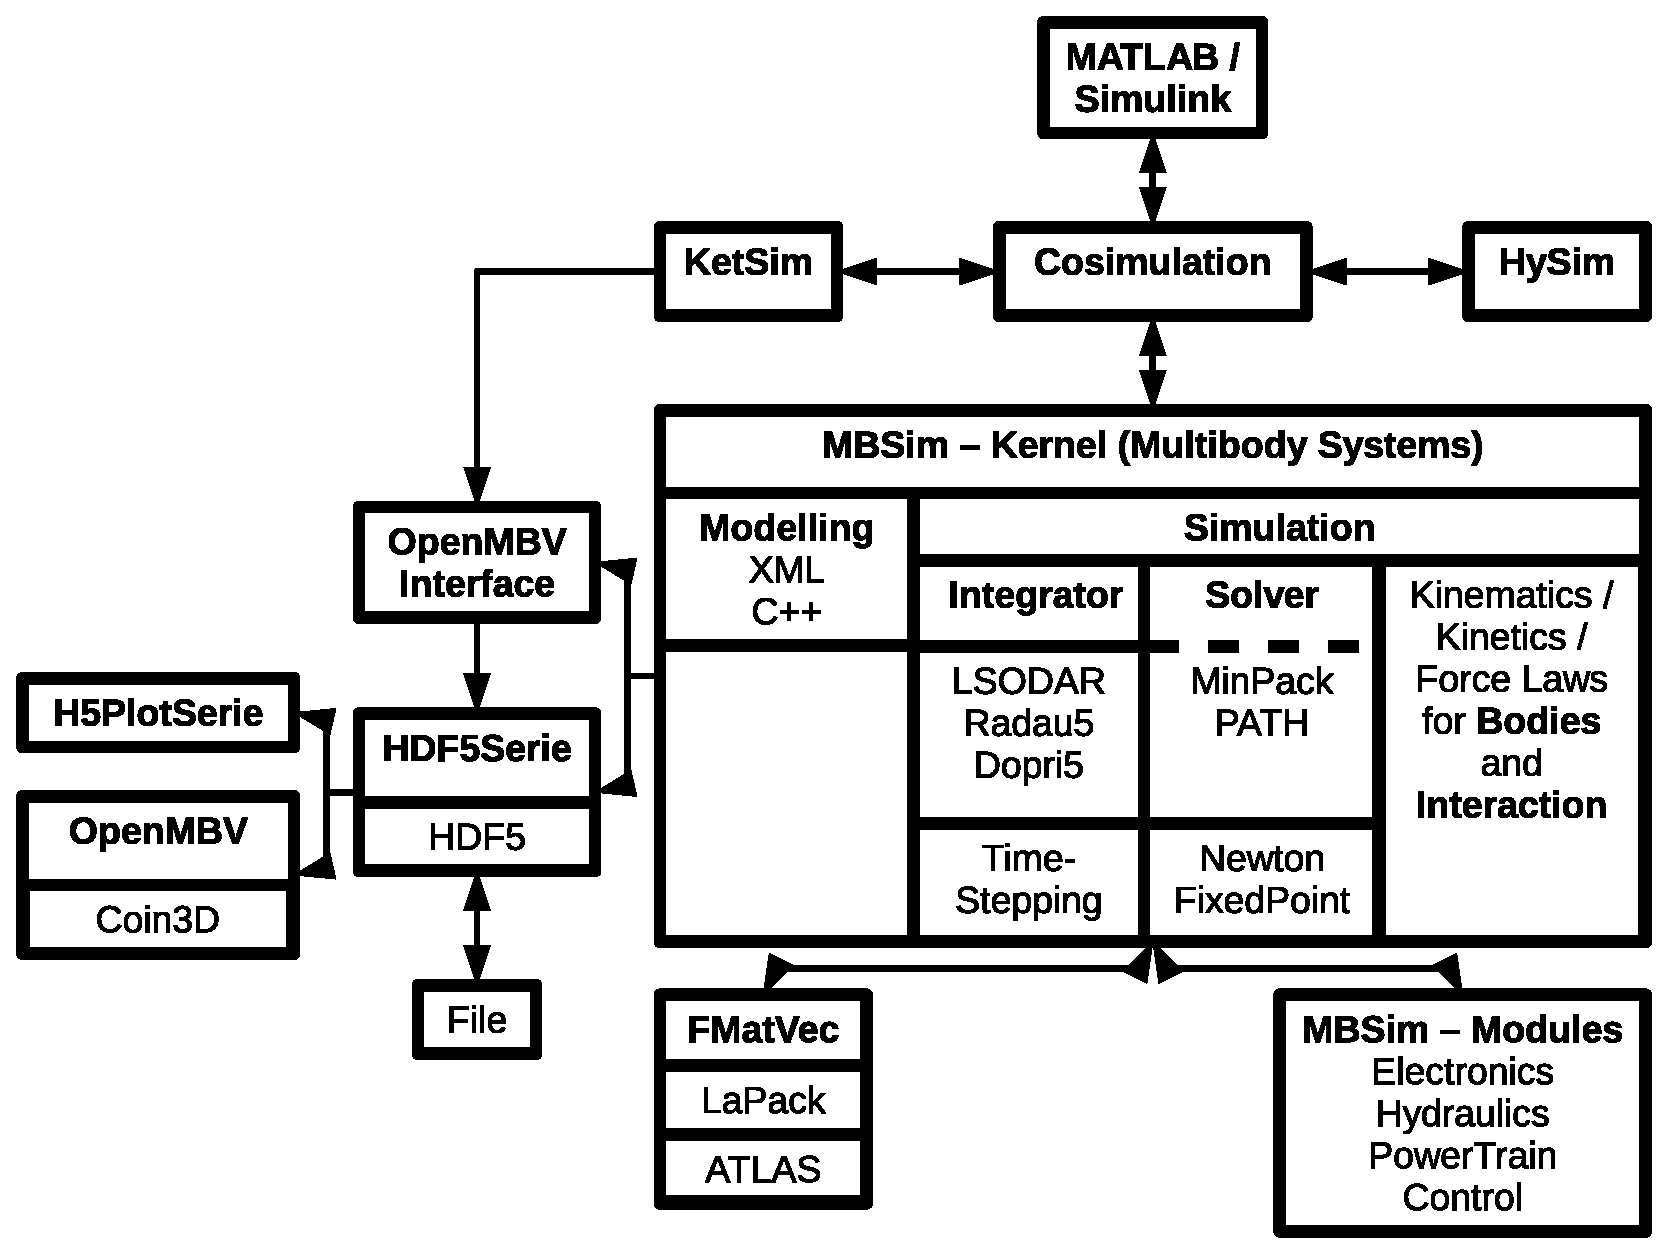
\includegraphics[width=0.9\hsize]{Figures/mbsim_embedding_grey.eps}
    \label{fig:departure:mbsim:embedding}
\end{figure}                                                                                                                                                                                                                                                                                                                                      
\MBSim{} can handle a set of dynamical systems from various domains not only separated but also exchanging data of the form
\begin{align*}
\dot{\vq}&=\vY\vu\,,\\
\vM\dot{\vu}&=\vh\left(\vq,\vu,t\right)+\vW\vlambda\,,\\
\dot{\vx}&=\vf\left(\vx\right)\,,\\
&\left(\vq,\vu,\vlambda,t\right)\in\mathcal{N}\,.
\end{align*}
Though, the simulation of hydraulics, electronics, control and power train systems is included within several modules. \MBSim{} is based on the interface \FMatVec{} using either LaPack\footnote{cf.~\url{http://www.netlib.org/lapack/}} or ATLAS\footnote{cf.~\url{http://www.netlib.org/atlas/}} for fast evaluation of linear algebra routines. Further, it uses \emph{HDF5Serie} to write files using the hierarchical HDF5 file format\footnote{cf.~\url{http://www.hdfgroup.org/HDF5/}} even for large dynamical systems. These files can be read by \emph{H5PlotSerie} for plotting or by \OpenMBV{} for visualisation. Thereby, \OpenMBV{} is based on the Coin implementation\footnote{cf.~\url{http://www.coin3d.org/}} of the Open Inventor Library\footnote{\url{http://oss.sgi.com/projects/inventor/}}. Also a co-simulation with Matlab/Simulink\footnote{cf.~\url{http://www.mathworks.de/}}, HySim \cite{Bor03} for hydraulic components and KetSim \cite{Fri98} for camshaft timing chains is possible. \MBSim{} is divided in a modelling part using C++ or XML and a simulation part. The simulation part is implemented quite modular distinguishing between the update of bodies and interactions concerning kinematics, kinetics as well as force laws and integration / nonlinear solution schemes. Also here external libraries are used where it is possible for having always a state-of-the-art numerical basis.
A typical example of a dynamical system only from mechanics is given by Figure~\ref{fig:objects}.
\begin{figure}[hbt]%
	\centering
    \footnotesize
    \psfrag{Body}{\texttt{Body}}
    \psfrag{Frame}{\put(+4.0,+0.0){\texttt{Frame}}}
    \psfrag{Contour}{\put(+2.0,+0.0){\texttt{Contour}}}
    \psfrag{Joint}{\texttt{Joint}}
    \psfrag{Contact}{\put(+2.0,+1.0){\texttt{Contact}}}
    \psfrag{Load}{\put(-50.0,+5.0){\texttt{KineticExcitation}}}
  	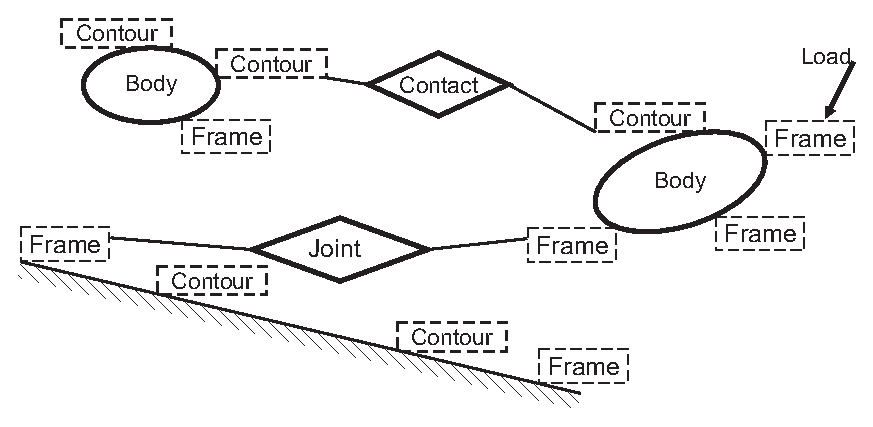
\includegraphics[width=0.9\hsize]{Figures/mbsim_objectorientation.eps} 
  	\caption{Object structure in \emph{MBSim}.}
  	\label{fig:objects}
\end{figure}
One has the environment and two \texttt{Object}s, in mechanics called \texttt{Body}s, holding the inertia terms. Indicated are interconnecting \texttt{Link}s due to \texttt{Contact}s between \texttt{Body} \texttt{Contour}s giving also the possibility to model friction and ideal \texttt{Joint}s between body \texttt{Frame}s as well as an external \texttt{KineticExcitation} acting on a body \texttt{Frame}. These ingredients from the mechanical point of view and a schedule of the simulation are basically explained in the following.

\subsection{Description of the Components}
The following classes can be used for modelling and simulating dynamical systems in \MBSim{}.

\subsubsection{DynamicSystem and DynamicSystemSolver}
Hierarchically objects and links belong to \texttt{DynamicSystem}s, which themselves can be \texttt{Group}ed (cf.~Figure~\ref{fig:departure:mbsim:dynamicsystem}). 
\begin{figure}[hbt]%
	\centering
    \footnotesize
  	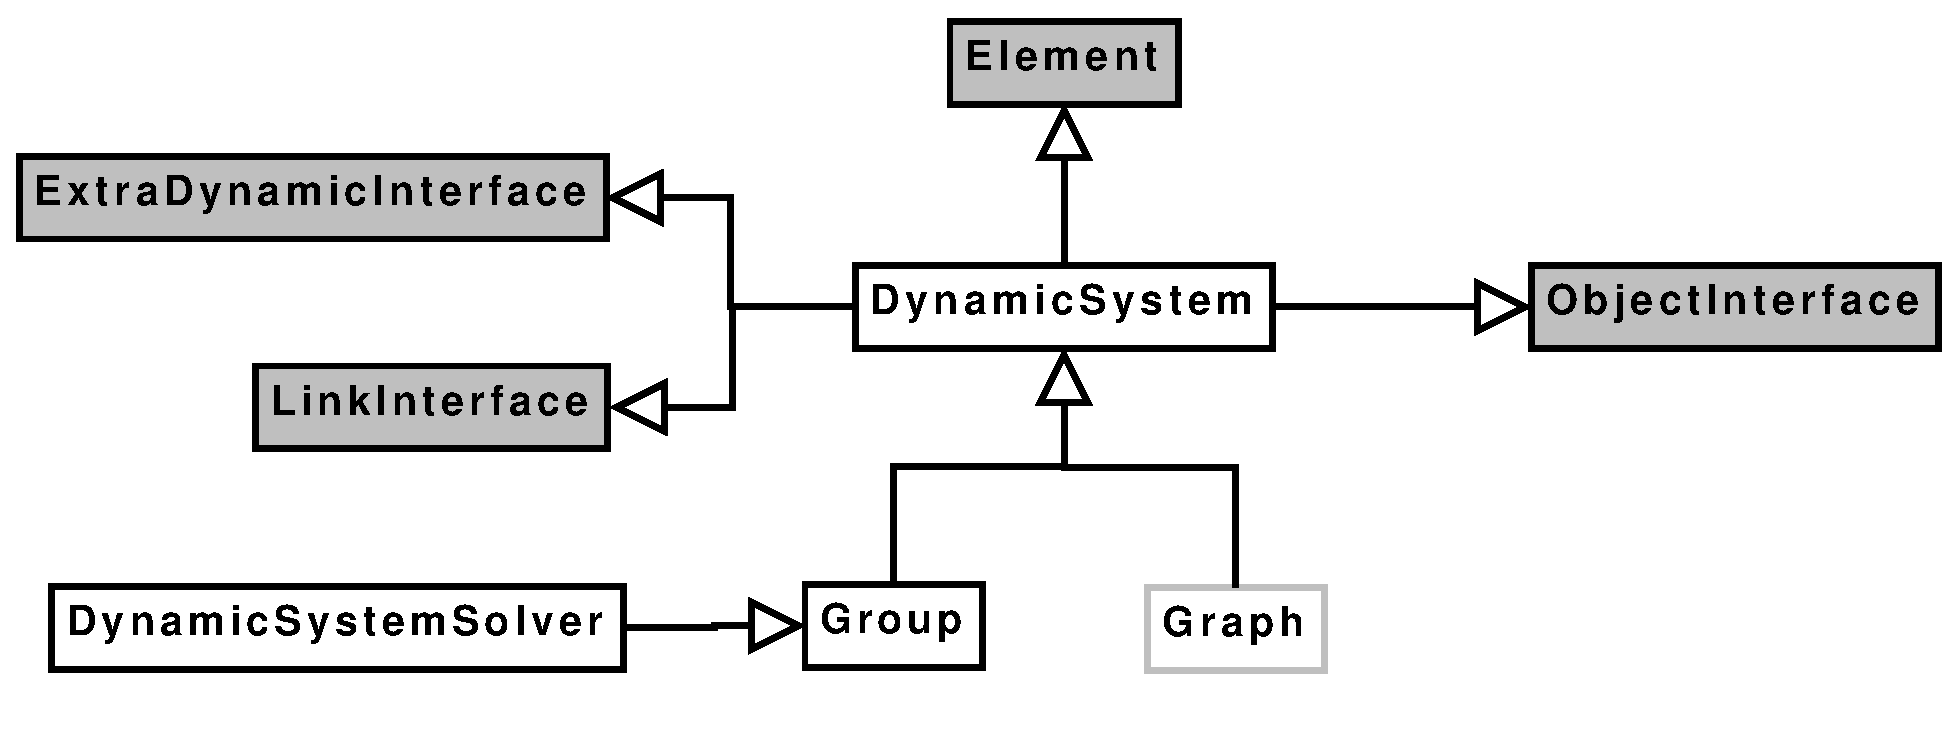
\includegraphics[width=0.7\hsize]{Figures/mbsim_dynamicsystem.eps} 
  	\caption{Dynamic system type classes in \MBSim{}.}
  	\label{fig:departure:mbsim:dynamicsystem}
\end{figure}
Shaded one can see interfaces for the different components of the modelling equations
\begin{itemize}
\item \texttt{ExtraDynamicInterface} 
  \begin{align}
  \dot{\vx}=\vf\left(\vx\right)
  \end{align}
\item \texttt{ObjectInterface}
  \begin{align}
  \dot{\vq}&=\vY\vu\,,\\
  \vM\left(\vq\right)\dot{\vu}&=\vh\left(\vq,\vu,t\right)\,,\,\vM\,\text{symmetric positive definite}
  \end{align}
\item \texttt{LinkInterface}
  \begin{align}
  &\left(\vq,\vu,\vlambda,t\right)\in\mathcal{N}\,,\\
  &\vh\left(\vq,\vu,t\right)\,,\vW\left(\vq\right)\vlambda
 \end{align} 
\end{itemize}
and \texttt{Element} for load/save mechanism as well as plot and data administration. Class \texttt{Graph} is dotted as it is not available for modelling. A graph structure is automatically built during initialisation for an efficient simulation process evaluating the hierarchical modelling structure. The top-most \texttt{DynamicSystem} is called \texttt{DynamicSystemSolver}. It also represents the interface to the integration schemes and allows the setting of environment variables (e.g. gravitation).\par
Important settings: 
\begin{itemize}
\item[] \texttt{addObject}\\
    add an \texttt{Object}, e.g. a \texttt{Body} from mechanics
\item[] \texttt{addLink}\\
    add a \texttt{Link}, e.g. a \texttt{Contact} or a \texttt{Joint} from mechanics
\item[] \texttt{addGroup}\\
    add a \texttt{DynamicSystem}
\item[] \texttt{addFrame}\\
    add a \texttt{Frame}
\item[] \texttt{addContour}\\
    add a \texttt{Contour}
\item[] \texttt{readz0}\\
    read initial state from \HDF{} file
\item[] \texttt{writez}\\
    write current state to \HDF{} file
\item[] \texttt{setReorganizeHierarchy}\\
    enforces the automatic creation of invisible graph structures only for simulation depending on the hierarchy of frames used for modelling 
\item[] \texttt{setConstraintSolver}\\
    solver for constraint equations on acceleration level (cf. \emph{setImpactSolver})
\item[] \texttt{setImpactSolver}\\
    solver for constraint equations on velocity level; available constraint equation solution schemes are
    \begin{itemize}
        \item[] \texttt{LinearEquations}\\
        Cholesky solution scheme for regular linear systems (only bilateral constraints)
        \item[] \texttt{GaussSeidel}\\
        Gauss-Seidel solution scheme for piecewise linear systems (planar Coulomb friction)
        \item[] \texttt{FixedPointSingle}\\
        Gauss-Seidel solution scheme with fixed point search and relaxation strategy (spatial Coulomb friction)
        \item[] \texttt{RootFinding}\\
        damped and globalised Newton scheme (spatial Coulomb friction)
        \end{itemize}
\item[] \texttt{setLinAlg}\\
    linear equations solver for \emph{RootFinding}; available solvers are
    \begin{itemize}
    \item[] \texttt{LUDecomposition}\\
    LU decomposition is only valid for non-singular contact situations
    \item[] \texttt{LevenbergMarquardt}\\
    regularisation of contact matrix by Levenberg Marquardt factor
    \item[] \texttt{PseudoInverse}\\
    selecting the norm-minimal solution if there exist several 
    \end{itemize}
\item[] \texttt{setStrategy}\\
    set relaxation strategy to \texttt{local} (contact wise) or \texttt{global} (all contacts)
\item[] \texttt{setNumJacProj}
\item[] \texttt{setMaxIter}\\
    set the maximum number of iterations in the contact solver
\item[] \texttt{setStopIfNoConvergence}\\
    the integrator stops integration, if there is no convergence in the contact solver
\end{itemize}
%
\subsubsection{Frames}
\texttt{Frame}s are a basic concept in the kernel of \MBSim{} to define an interface for \MBSim{} multibody components concerning kinematic and kinetic expressions. New \texttt{Frame}s can be added arbitrarily and recursively based on a predecessor \texttt{Frame}. That is why there has to be a first \texttt{Frame} for specific \MBSim{} components, e.g. each \texttt{DynamicSystem} has got a stationary \texttt{Frame} \texttt{"I"} (inertia frame).\par
Important settings next to position and Cartesian orientation are defined according to the parametrisation
\begin{align*}
  	\begin{pmatrix}	\rs{_I}[_P]{\va}\\ \rs{_I}{\vPsi}\end{pmatrix} 
	&= \begin{pmatrix}\rs{_I}[_P]{\vJ}\\ \rs{_I}[_R]{\vJ}\end{pmatrix} \,
	\dot{\vu} +
   	  \begin{pmatrix}\rs{_I}[_P]{\viota}\\\rs{_I}[_R]{\viota}\end{pmatrix}
\end{align*}
of translational and angular acceleration. This is basically an affine relationship concerning the derivative of generalised velocities $\dot{\vu}$, appropriate \textsc{Jacobian} matrices and an explicit time dependent summand.
Summarizing
\begin{itemize}
\item[] \texttt{getPosition} 
\item[] \texttt{getOrientation} 
\item[] \texttt{getVelocity}
\item[] \texttt{getAngularVelocity} 
\item[] \texttt{getJacobianOfTranslation} 
\item[] \texttt{getJacobianOfRotation}
\item[] \texttt{getGyroscopicAccelerationOfTranslation}
\item[] \texttt{getGyroscopicAccelerationOfRotation}
\item[] \texttt{enableOpenMBV}\\
    enabling visualisation for \OpenMBV{}
\end{itemize}
are important settings.
%
\subsubsection{Bodies}
Mechanical \texttt{Body}s provide their portion of a positive definite mass matrix, a smooth right hand side, state and energy expressions according to \texttt{Object}, which is e.g. similar to some hydraulic objects (cf.~Figure~\ref{fig:departure:mbsim:object}).
\begin{figure}[hbt]%
	\centering
    \footnotesize
  	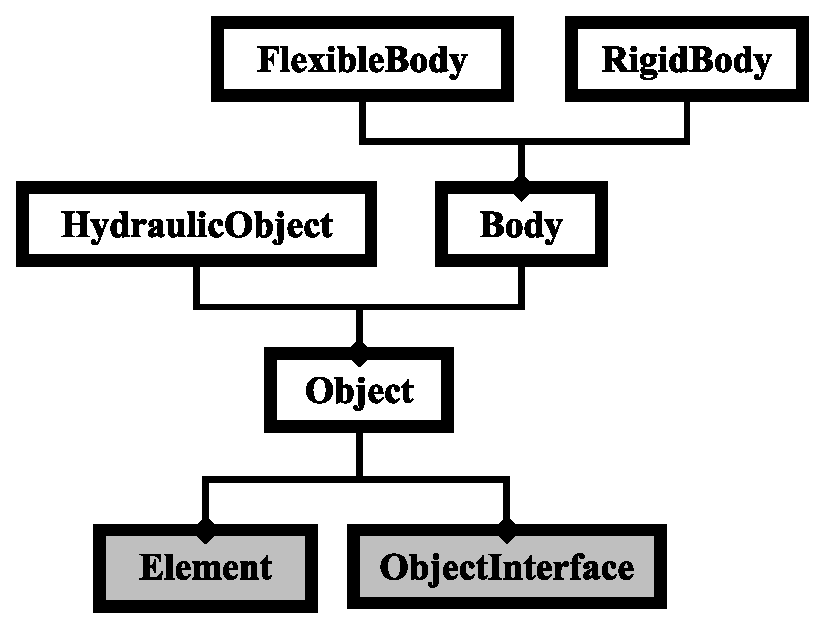
\includegraphics[width=0.45\hsize]{Figures/mbsim_object.eps} 
  	\caption{Object type classes in \MBSim{}.}
  	\label{fig:departure:mbsim:object}
\end{figure}
Different is the kinematic description which is based on \texttt{Frame}s in the case of mechanical \texttt{Body}s. Also the connectors to other \texttt{Body}s might follow other structural rules. Depending on the type of linkage \texttt{Frame}s or \texttt{Contour}s occur in the case of \texttt{Body}s.\par
Important settings: 
\begin{itemize}
\item[] \texttt{addFrame}\\
    add a \texttt{Frame}
\item[] \texttt{addContour}\\
    add a \texttt{Contour}
\end{itemize}

\paragraph{Rigid Bodies}
For each \texttt{RigidBody} a \texttt{Frame} \texttt{"C"} in the centre of gravity is predefined. One perhaps newly created \texttt{Frame} of the \texttt{RigidBody} has to be chosen as frame for kinematics \texttt{"K"} with centre $P$ and one \texttt{Frame} of another \texttt{Body} or a \texttt{DynamicSystem} has to be chosen as frame of reference \texttt{"R"} with centre $O'$. Both absolute --if the frame of reference belongs to a \texttt{DynamicSystem}-- and relative --if the frame of reference belongs to another \texttt{RigidBody}-- kinematic structures are canonically given by the frame recursion. The motion of the frame of kinematics and so also the \texttt{RigidBody} with respect to the frame of reference is defined by the individual generalised coordinates ${\vq}_{\text{rel}}$ of the \texttt{RigidBody} or its constrained relative motion. These settings can be defined individually on position, velocity and acceleration level according to
\begin{align}
        \rs{_R}[_{O'P}]{\vr} &= \rs{_R}[_{O'P}]{\vr}({\vq}_{\text{rel}},\,t)\,,\\
        \vA_{RK} &= \vA_{RK}({\vq}_{\text{rel}},\,t)\,,\\
        \rs{_R}[_{O'P,\text{rel}}]{\vv} &=  \rs{_R}[_{P,\text{rel}}]{\vJ} \,\vu_\text{rel} + \rs{_R}[_{P,\text{rel}}]{\viota}  \, \\
        \rs{_R}[_{RK}]{\vomega} &= \rs{_R}[_{R,\text{rel}}]{\vJ} \,\vu_\text{rel} + \rs{_R}[_{R,\text{rel}}]{\viota} \\
        \frac{\mathrm{d}}{\mathrm{d} t}\left(\rs{_R}[_{O'P,\text{rel}}]{\vv}\right) &= \rs{_I}[_{P,\text{rel}}]{\vJ} \,\dot{\vu}_\text{rel} +\frac{\mathrm{d}}{\mathrm{d} t}\left(\rs{_R}[_{P,\text{rel}}]{\vJ} \right)\,\vu_\text{rel} + \frac{\mathrm{d}}{\mathrm{d} t}\left(\rs{_R}[_{P,\text{rel}}]{\viota} \right)  \,,\\ 
        \frac{\mathrm{d}}{\mathrm{d} t}\left(\rs{_R}[_{RK}]{\vomega}\right) &= \rs{_I}[_{R,\text{rel}}]{\vJ} \,\dot{\vu}_\text{rel} +\frac{\mathrm{d}}{\mathrm{d} t}\left(\rs{_R}[_{R,\text{rel}}]{\vJ} \right)\,\vu_\text{rel} + \frac{\mathrm{d}}{\mathrm{d} t}\left(\rs{_R}[_{P,\text{rel}}]{\viota} \right)
\end{align}
and Figure~\ref{fig:departure:mbsim:rigid_kinematics} also including the link relationships of frames and contours.
\begin{figure}[hbt]%
	\centering
    \footnotesize
    \psfrag{DS}{\texttt{DynamicSystem}}
    \psfrag{RB}{\texttt{RigidBody}}
    \psfrag{link}{\texttt{Link}}
    \psfrag{C}{\put(+0.0,+0.0){$C$}}
    \psfrag{Itilde}{\put(+0.0,+0.0){$\tilde{I}$}}
    \psfrag{I}{\put(+0.0,+0.0){$I$}}
    \psfrag{B}{\put(+0.0,+0.0){$B$}}
    \psfrag{q}{\put(+0.0,+0.0){$q_{\text{rel}}$}}
  	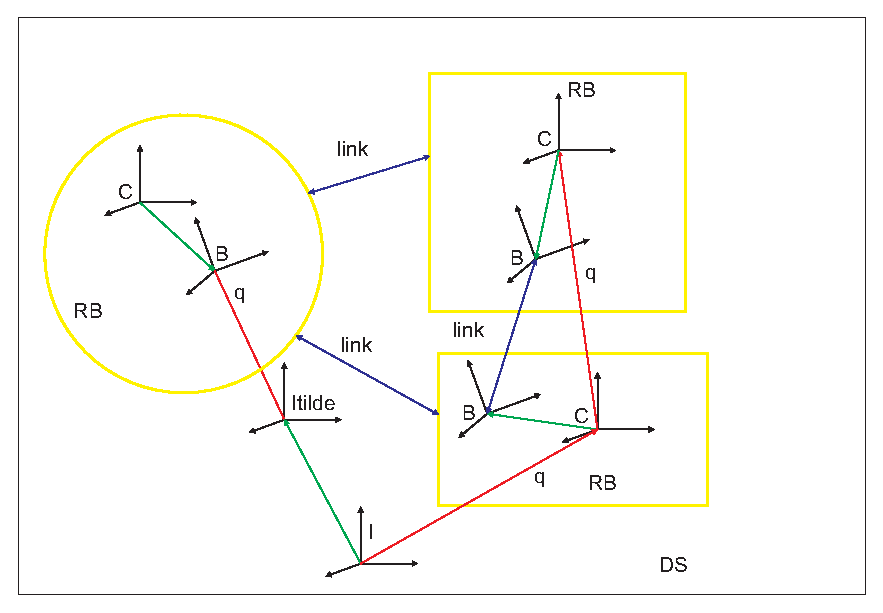
\includegraphics[width=0.6\hsize]{Figures/mbsim_rigid_kinematics.eps} 
  	\caption{Rigid kinematics in \MBSim{}.}
  	\label{fig:departure:mbsim:rigid_kinematics}
\end{figure}
The drawback of this general description is a time-dependent mass-matrix also in the absolute kinematics case.\par
Important settings: 
\begin{itemize}
\item[] \texttt{setMass}
\item[] \texttt{setInertiaTensor}\\
    is defined with respect to \texttt{"C"}, if no other \texttt{Frame} is given as second argument
\item[] \texttt{setFrameOfReference}\\
    one possibility to define initial values
\item[] \texttt{setFrameForKinematics}
\item[] \texttt{setOpenMBVRigidBody}\\
    enabling visualisation for \OpenMBV{}
\end{itemize}
Kinematics can be defined individually using the member functions
\begin{itemize}
\item[] \texttt{setTranslation}
\item[] \texttt{setRotation}
\item[] \texttt{setJacobianOfTranslation}
\item[] \texttt{setJacobianOfRotation}
\item[] \texttt{setDerivativeOfJacobianOfTranslation}
\item[] \texttt{setDerivativeOfJacobianOfRotation}
\item[] \texttt{setGuidingVelocityOfTranslation}
\item[] \texttt{setGuidingVelocityOfRotation}
\item[] \texttt{setDerivativeOfGuidingVelocityOfTranslation}
\item[] \texttt{setDerivativeOfGuidingVelocityOfRotation}
\end{itemize}
For convenience it is sometimes not necessary to define all components. E.g. for a \texttt{LinearTranslation} as well as \texttt{RotationAboutFixedAxis} and \texttt{CardanAngles} everything else is derived automatically.

\paragraph{Flexible Bodies}
The equations of motion of a \texttt{FlexibleBody} is at the moment only available with respect to a stationary \texttt{Frame}. So, for flexible bodies the frame of reference must belong to a \texttt{DynamicSystem}. The following flexible bodies are available. 

\begin{itemize}
%\item \emph{BodyFlexible1s01Torsion}
%\item \emph{BodyFlexible1s21ANCF} 2D-Balken mit Absolute Nodal Coordinate Formulation
\item[] \texttt{FlexibleBody1s21RCM}\\
  planar beam using redundant coordinate methode with three coordinates per finite element node, translation  $x$, $y$ and rotation $\gamma$, as well as two additional bending deflections $c_1$, $c_2$
\item[] \texttt{FlexibleBody1s33RCM}\\
  spatial beam using redundant coordinate methode with six coordinates per finite element node, translation  $x$, $y$, $z$ and reversed Cardan rotation $\alpha$, $\beta$, $\gamma$, as well as four additional bending deflections $c_1$, $c_2$, $c_3$, $c_4$
%\item \emph{BodyFlexible1s23BTA} Biege-Torsions-Welle (5-Koordinaten pro Knoten $\alpha$, $y$, $\gamma$, $z$, $\beta$ im jeweils mit $\alpha$ mitdrehenden KOSY)
%\item \emph{BodyFlexibleLinearExternal}
\end{itemize}

\subsubsection{LinkMechanics}
\texttt{LinkMechanics} represents interconnections between mechanical bodies according to Figure~\ref{fig:departure:mbsim:link} using the connectors of \texttt{Body}s. 
\begin{figure}[hbt]%
	\centering
    \footnotesize
  	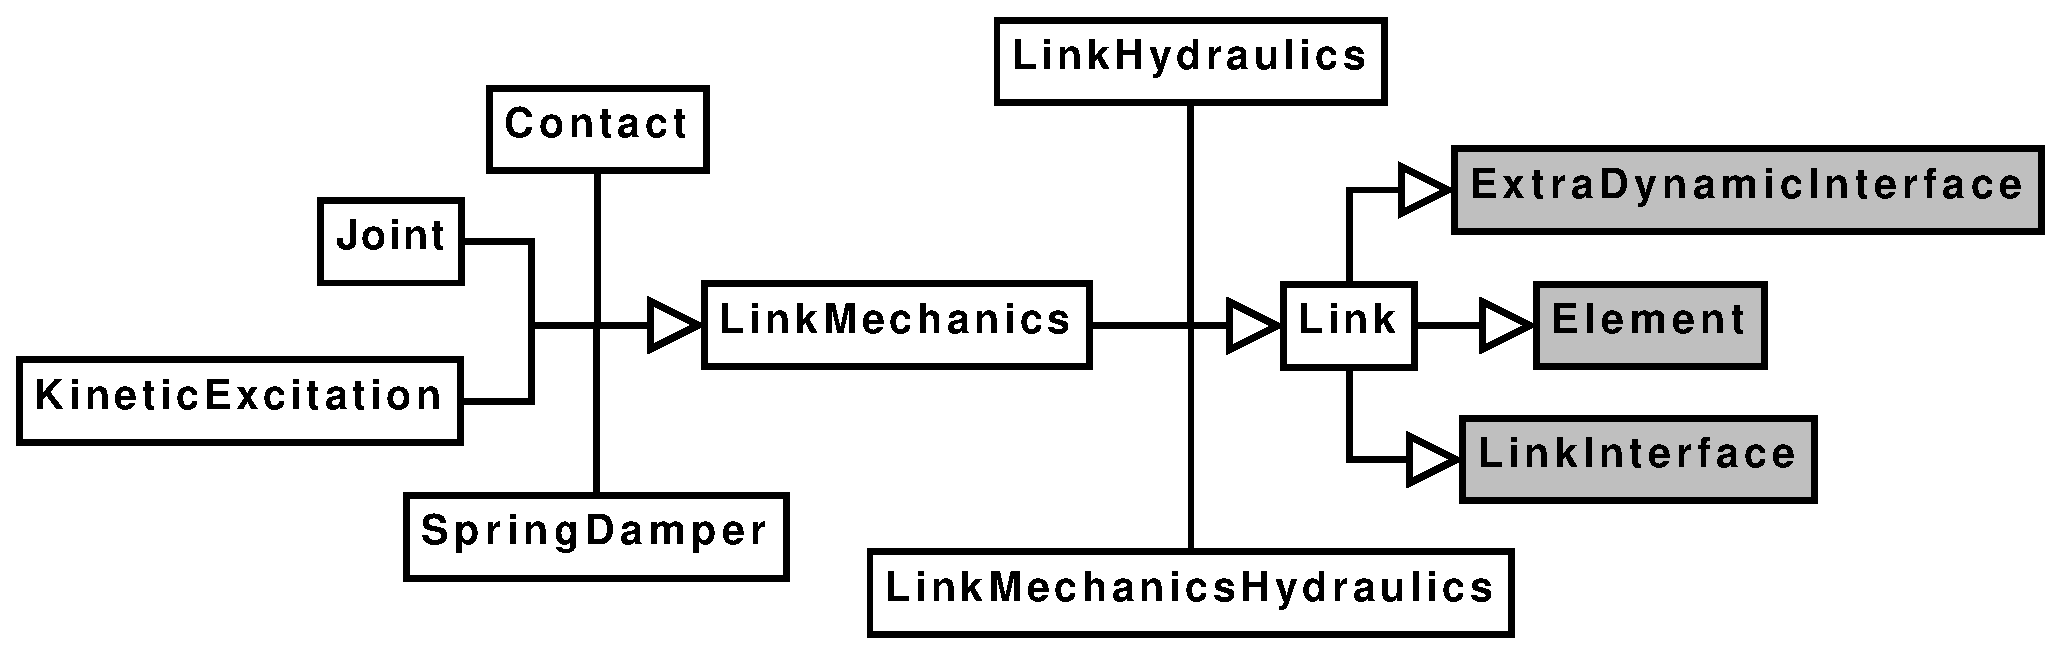
\includegraphics[width=0.8\hsize]{Figures/mbsim_link.eps} 
  	\caption{Link type classes in \MBSim{}.}
  	\label{fig:departure:mbsim:link}
\end{figure}
If other connectors are used other link classes have to be inherited. Always \texttt{Link}s distribute locally to $\vh$ and $\vW\vlambda$ in the equations of motion.\par
Important settings: 
\begin{itemize}
\item[] \texttt{connect}\\
    connect mechanical links to \texttt{Frame}s
\item[] \texttt{setOpenMBVForceArrow}\\
    visualisation of link forces in \OpenMBV{}
\item[] \texttt{setOpenMBVMomentArrow}\\
    visualisation of link torques in \OpenMBV{}
\end{itemize}
%
\paragraph{SpringDamper}
A \texttt{SpringDamper} connects two \texttt{Frame}s using a predefined spring force function.\par
Important settings: 
\begin{itemize}
\item[] \texttt{setForceFunction}
\item[] \texttt{setProjectionDirection}\\
    projection direction of the force, if it should not act in direction of the \texttt{Frame}s' connecting vector
\item[] \texttt{setOpenMBVSpring}\\
    visualisation of a spring in \OpenMBV{}
\end{itemize}

\paragraph{KineticExcitation}
A \texttt{KineticExcitation} is connected to one \texttt{Frame} using a predefined excitation function.\par
Important settings: 
\begin{itemize}
\item[] \texttt{setForce}\\
    force excitation function
\item[] \texttt{setMoment}\\
    moment excitation function
\item[] \texttt{setFrameOfReference}\\
    force / moment direction vectors, if not the connected \texttt{Frame} should be used
\end{itemize}

\paragraph{Joints}
\texttt{Joint}s connect two \texttt{Frame}s with the force laws depending on the ideal normal relative kinematics. The constitutive law has to be chosen for the calculation of the force parameter.\par
Important settings: 
\begin{itemize}
\item[] \texttt{setForceDirection}\\
    constraint force directions
\item[] \texttt{setMomentDirection}\\
    constraint moment directions
\item[] \texttt{setForceLaw}\\
    constitutive law on acceleration level
\item[] \texttt{setImpactForceLaw}\\
    constitutive law on velocity level
\end{itemize}

\paragraph{Contacts and Impacts}
Contacts and impacts are managed by class \texttt{Contact}.\par
Important settings: 
\begin{itemize}
\item[] \texttt{setContactForceLaw}\\ 
    constitutive normal law on acceleration level
\item[] \texttt{setContactImpactLaw}\\
    constitutive normal law on velocity level
\item[] \texttt{setFrictionForceLaw}\\
    constitutive friction law on acceleration level
\item[] \texttt{setFrictionImpactLaw}\\
    constitutive friction law on velocity level
\item[] \texttt{setContactKinematics}\\
    The relative kinematics is defined between \texttt{Contour} classes. On velocity level the contact kinematics is independent of the specific contour. For the calculations on position level the following contours are available.
    \begin{itemize}
    \item[] \texttt{CircleHollow}\\
        one dimensional sphere with contact from inside 
    \item[] \texttt{CircleSolid}\\
        one dimensional sphere with contact from outside 
    \item[] \texttt{FlexibleBand}\\
        flexible contour describing a band in a certain distance and direction of a neutral fibre
    \item[] \texttt{Frustum}\\
        frustum with its axis given by the second column of the contour reference frame
    \item[] \texttt{Line}\\
        affine one dimensional space 
    \item[] \texttt{Plane}\\
        affine two dimensional surface
    \item[] \texttt{Point}\\
        most primitive rigid contour
    \item[] \texttt{Sphere}\\
        two dimensional sphere
    \end{itemize}
    Each contour has a contour fixed frame, with the third column of the orientation matrix being the binormal for planar contours and the first column being the normal of linear contours. Sometimes they can be visualised with \texttt{enableOpenMBV}.\par
    Available contact kinematics on position level:
    \begin{itemize}
    \item[] \texttt{CircleFrustum}
    \item[] \texttt{CircleSolidLine}
    \item[] \texttt{PointLine}
    \item[] \texttt{PointFrustum}
    \item[] \texttt{PointPlane}
    \item[] \texttt{PointFlexibleBand}
    \item[] \texttt{SphereFrustum}
    \item[] \texttt{SpherePlane}
    \end{itemize}

\item[] \texttt{enableOpenMBVContactPoints}\\
    enables the visualisation of accompanying contact frames in \OpenMBV{}
\item[] \texttt{setOpenMBVNormalForceArrow}\\
    visualisation of the normal force arrow in \OpenMBV{}
\item[] \texttt{setOpenMBVFrictionArrow}\\
    visualisation of the friction force arrow in \OpenMBV{}
\end{itemize}

\paragraph{Constitutive Laws}
Concerning the constitutive laws it is distinguished between contact laws on acceleration and impact laws on velocity level. Further, both flexible and rigid laws in normal and tangential direction are available.\footnote{Modelling hint: There are contradictions between energy conservation in normal direction and dissipation due to friction when combining these features.}\par
Important possibilities:
\begin{itemize}
\item[] \texttt{UnilateralConstraint}\\
    set-valued on acceleration level
\item[] \texttt{BilateralConstraint}\\
    set-valued on acceleration level
\item[] \texttt{UnilateralNewtonImpact}\\
    set-valued on velocity level
\item[] \texttt{BilateralImpact}\\
    set-valued on velocity level
\item[] \texttt{PlanarCoulombFriction}\\
    set-valued on acceleration level
\item[] \texttt{SpatialCoulombFriction}\\
    set-valued on acceleration level
\item[] \texttt{PlanarStribeckFriction}\\
    set-valued on acceleration level
\item[] \texttt{SpatialStribeckFriction}\\
    set-valued on acceleration level
\item[] \texttt{PlanarCoulombImpact}\\
    set-valued on velocity level
\item[] \texttt{SpatialCoulombImpact}\\
    set-valued on velocity level
\item[] \texttt{PlanarStribeckImpact}\\
    set-valued on velocity level
\item[] \texttt{SpatialStribeckImpact}\\
    set-valued on velocity level
\item[] \texttt{RegularizedUnilateralConstraint}\\
    single-valued on acceleration level
\item[] \texttt{RegularizedBilateralConstraint}\\
    single-valued on acceleration level
\item[] \texttt{RegularizedPlanarFriction}\\
    single-valued on acceleration level
\item[] \texttt{RegularizedSpatialFriction}\\
    single-valued on acceleration level
\end{itemize}

\paragraph{Conventions}
For modelling own contact kinematics and constitutive laws some conventions are important.
\begin{itemize}
\item contact kinematics\\
    \texttt{updateg} should define the normal distance, the possible contact locations and trihedral orientations, \texttt{updatewb} are nonlinear kinematic terms on acceleration level
\item accompanying contour trihedral\\
    the first column is the outward pointing normal, then the two tangentials follow with only the first tangent-pair having opposite sign 
\end{itemize}

\subsubsection{Functions}
Depending on the number of arguments it is possible to derive new functions from \texttt{Function1}, \texttt{Function2} and \texttt{Function3} by specifying the template parameters. They are used at various places and are a general way of re-using functional descriptions.

\subsubsection{Integration Schemes}
Available integration schemes:
\begin{itemize}
\item[] \texttt{DOPRI5Integrator}\\
    Dormand-Prince one-step integration scheme of order 5 for nonstiff ODE with step size control
\item[] \texttt{RADAU5Integrator}\\
    one-step integration scheme of order 5 for stiff ODE with step size control
\item[] \texttt{TimeSteppingIntegrator}\\
    one-step semi-implicit integration scheme of order 1 for nonstiff MDE
\item[] \texttt{ThetaTimeSteppingIntegrator}\\
    one-step integration scheme of order 1 for nonstiff with $\Theta=0$ and stiff with $\Theta\in\left(0,1\right]$ MDE
\end{itemize}
%DAEs behandeln \emph{RADAU5DAEIntegrator}, \emph{DASKRIntegrator} und \emph{DASPKIntegrator}. Dar\"uberhinaus gibt es noch \emph{RKSuite}, \emph{LSODAR} (Mehrschrittverfahren steif/nicht steif) und \emph{LSODE}.  \emph{TimeSteppingSSCIntegrator} implementiert f�r den semi-impliziten Fall eine Schrittweitensteuerung und \emph{DAETSIntegrator} liefert eine Kopplung zwischen TimeStepping und Dassl. 

\subsection{Program Flow}
Conceptionally the program flow is defined by the election of the integration scheme. It can always be stopped using \texttt{Ctrl-C} also enforcing the closing of the plot functionality. With
\begin{verbatim}
kill -USR2 <PID of simulation thread>
\end{verbatim}
a flush of the plot routine is asked for.

\subsubsection{Timestepping Integration}
Timestepping integration solves the whole equations of the system including the contacts on velocity level with fixed time step size. In detail one has the following work flow.
\begin{enumerate}
\item $\text{\texttt{DS::plot}}\left(t,\vq,\vu\right)$
\item $\vq\leftarrow\vq+\text{\texttt{DS::deltaq}}\left(t,\vq,\vu\right)$
\item $t\leftarrow t+\Delta t$
\item $\text{\texttt{DS::update}}\left(t,\vq,\vu\right)$
    \begin{enumerate}
    \item[]\texttt{DS::updateStateDependentVariables}\\
      update variables depending on the generalised state and the structure of the system with one independent group and several recursive calculation graphs
    \item[]\texttt{DS::updateg}
      \begin{itemize}
      \item update of the relative position kinematics independent of the system structure using the order
      \begin{align*}
        \text{\texttt{Link}}\rightarrow\text{\texttt{LinkMechanics}}\left(\rightarrow\text{\texttt{ContactKinematics}}\right)
      \end{align*}
      \item several contacts points are possible from the kinematical point of view, whereby the maximum number is calculated in \texttt{ContactKinematics}\\
      \end{itemize}
    \item[]\texttt{DS::checkActiveg}
      \begin{itemize}
      \item determine the state of the relative kinematics concerning the activity of links
      \item redefine global memory references using indices 
      \end{itemize}
    \item[]\texttt{DS::updategd}
      \begin{itemize}
      \item update of the relative velocity kinematics independent of the system structure
      \item can be done in the child classes of \texttt{LinkMechanics}
      \end{itemize}
    \item[]\texttt{DS::updateT}\\
      updates the linear transformation matrix $\dot{\vq}=\vT\vu$ independent of the system structure
    \item[]\texttt{updateJacobians}\\
      updates the \textsc{Jacobians} for projecting forces in generalised directions dependent on the system structure
    \item[]\texttt{updateh}\\
      updates the right hand sides with the possibility to account for internal forces of \texttt{objects} and external forces of \texttt{links} independent of the system structure
    \item[]\texttt{updateM}\\
      updates the mass matrix independent of the system structure
    \item[]\texttt{facLLM}
      \begin{itemize}
      \item computes the \textsc{Cholesky} decomposition of the mass matrix dependent on the system structure
      \item \texttt{group} calculates the matrix inverse locally per object
      \item \texttt{graph} calculates the matrix inverse globally
      \end{itemize}
    \item[]\texttt{updateW}\\
      updates the \textsc{Jacobian} between in general set-valued \texttt{link}-force parameters and generalised coordinates
    \item[]\texttt{updateV}
      \begin{itemize}
      \item the decomposition of the in general set-valued \texttt{link}-forces
      \begin{align*}
      \vW\vlambda=\vW_N\vlambda_N+\vW_T\vlambda_T
      \end{align*}
      in a normal and tangential part allows to separate the single-valued slip case
      \item for affected \texttt{links} it is
      \begin{align*}
      \tilde{\vW}\tilde{\vlambda}=\left(\tilde{\vW}_N+\mu\tilde{\vW}_T\right)\tilde{\vlambda}_N=\tilde{\vV}\tilde{\vlambda}_N\ .
      \end{align*}
      \item altogether this is a reduction of the set-valued equations being expressed by the projection
      \begin{align*}
      \vV\vlambda^{*}\ .
      \end{align*}
      \end{itemize}
    \item[]\texttt{updateG}
      \begin{itemize}
      \item the force action matrix
      \begin{align*}
      \vG=\vW^T\vM^{-1}\vV
      \end{align*}
      must be calculated by the most global view, namely the \texttt{DynamicSystemSolver}
      \item the size of $\vG$ is reduced due to the introduction of $\vV$ but is non-symmetric
      \item for a time-stepping scheme it is $\vV=\vW$
      \end{itemize}
    \end{enumerate}
\item $\text{\texttt{DS::solveImpacts}}\left(t,\vq,\vu\right)$
    \begin{itemize}
    \item the constrained equations are solved on velocity level using sparse matrix structures (cf.~\cite[MKL sparse matrix storage format]{Intel08})
    \item block structures are not evaluated
    \end{itemize}
\item $\vu\leftarrow\vu+\text{\texttt{DS::deltau}}$
\item $\vx\leftarrow\vx+\text{\texttt{DS::deltax}}$
\item \texttt{DS::projectGeneralizedPositions}
\end{enumerate}

\subsubsection{Event-Driven Integration}
Currently, \texttt{LSODAR} is the only event-driven integrator with automatic switch between stiff and non-stiff equations.
\begin{enumerate}
\item \texttt{DS::computeInitialCondition}\\
    checks for system configuration and creates the necessary contact container
\item $\text{\texttt{DS::plot}}\left(t,\vq\right)$
\item \texttt{DLSODAR} 
    \begin{enumerate}
    \item[]$\text{\texttt{DS::zdot}}\left(t,\vq,\vu\right)$ is available for standard and inverse kinetics calculations
      \begin{itemize}
      \item \texttt{wb} means $\bar{w}$ and describes the acceleration terms in the constraint kinematics
      \item \texttt{computeConstraintForces} uses a least square algorithm to solve the Delassus equations, assume $Ax=b$ with a $m\times n$ full-rank matrix $A$, then there are two cases
        \begin{itemize}
        \item $m\geq n$ (skinny) can always be solved by $\left\|Ax-b\right\|\rightarrow\min$ and so by SVD\\
          analytically the solution is given by the normal equations $x=\left(A^TA\right)^{-1}A^Tb$
        \item $m<n$ (fat) has an infinite dimensional solution space, one has to pick one solution\\
          $\left\|x\right\|\rightarrow\min,\ Ax=b$ which is analytically given by $x=A^T\left(A^TA\right)^{-1}b$, again numerically a SVD solves the problem most efficiently
        \end{itemize}
      \end{itemize}
    \item[]\texttt{DS::getsv} the stop vector defines the root function concerning contacts and stick-slip-transitions for the DAE solver
      \begin{itemize}
      \item it can be only set by \texttt{Link}
      \item contains kinematics for not-active directions and kinetics for active directions
      \item the last entry is used for position and velocity projections
      \item is solved by integrator concerning a tolerance
      \end{itemize}
    \end{enumerate}
\item \texttt{DS::shift} is invoked, if there is a sign change in the stop vector
    \begin{itemize}
      \item drift compensation if indicated by stop vector
      \item project to slighly positive gaps to avoid instantaneous appearance of new shift point
      \item \texttt{updateCondition} should impact or differential equations be solved, after earlier mentioned reconfiguring?
      \item case studies
        \begin{itemize}
        \item[] \texttt{impact} has highest priority and changes overall configuration
        \item[] \texttt{impact} requires \texttt{D::checkAllgd} because of possible slip-stick transition
        \item no difference between $\Lambda$ and $\lambda$
        \item \texttt{gdn} means $\dot{g}^{+}$
        \item[] \texttt{impact} involves new configuration and so also the equations of motion have to be solved
        \item \texttt{checkActivegdd} has to be done with the same tolerance like in the nonlinear equations solver
        \item[] \texttt{gActive} means a contact is closed
        \item[] \texttt{gdActive} means a contact remains closed
        \end{itemize}
    \end{itemize}
\end{enumerate}

%%------------------------------------------------------------ SUBSECTION --
\subsection{Plot Routines}\label{sec:plot}

\subsubsection{Usage}
The result of a simulation with \MBSim{} are a \texttt{mbsim.h5} file for plot analysis as well as \texttt{ombv.h5} and \texttt{ombv.xml} files for visualisation. Additionally there is information concerning the integrator in \texttt{*.plt} and \texttt{*.sum} files; for visualisation \texttt{*.iv} files might appear.\\
For getting data from \MBSim{} a \HDF{} wrapper is used. Plotting the multibody system data can be done with
\begin{verbatim}
    h5plotserie <h5-file>
\end{verbatim}
The usage is quite canonic and documented in the online help. Interesting features are
\begin{itemize}
\item superimposing graphs by \texttt{<shift>} and left click in the data list ,
\item change axes by \texttt{<ctrl>} and left click in the curve list ,
\item disabling graphs by right click in the curve list .
\end{itemize}
With
\begin{verbatim}
    h5lsserie <h5-file>
\end{verbatim}
basically the content can be shown. Several possible options are explained by typing \texttt{-h}:
\begin{enumerate}
\item[\texttt{-d}] shows the description of the data to plot
\item[\texttt{-l}] shows the column labels of the data to plot
\item[\texttt{-f}] follows external links in a set of \HDF{}-files to avoid redundant data (\HDF{} is possible per DynamicSystem)
\end{enumerate}
The specific names in \HDF{} format are specialised by reading from right to left. The url to specific data is given by a path and can be used in
\begin{verbatim}
    h5dumpserie <path>
\end{verbatim}
perhaps also in other tools. The column one is interested in is declared using a colon. Also several columns can be appended, whereby shorter ones are enlarged by \texttt{nan} entries. Altogether, it is possible to use the dump by
\begin{verbatim}
    gnuplot "<dump" u *:* w l
\end{verbatim}
or in \textsf{MatLab} by
\begin{verbatim}
    h5dump('<path>')
\end{verbatim}
\OpenMBV{} files can be openen by just typing \texttt{openmbv} in the specific directory. The usage should be quite canonic and is explained in the online help.


\subsubsection{Implementation}
In \MBSim{} plotting is done using \texttt{plotFeatures} being defined in \texttt{element.h}. They are set in \texttt{dynamic\_system\_solver.cc}. One plot-file comprises time-series of rowvectors with the same data type in all entries.

